\documentclass{beamer}

\newcommand{\lesson}{{\tt Linked Lists}}

\author[Chris Simpkins]
{Christopher Simpkins \\\texttt{chris.simpkins@gatech.edu}}
\institute[Georgia Tech] % (optional, but mostly needed)

\date[CS 1331]{}


\newcommand{\course}{Introduction to Object-Oriented Programming}
\subject{\course}
\title[\lesson]{\course}
\subtitle{\lesson}

\author[CS 1331]
{Christopher Simpkins \\\texttt{chris.simpkins@gatech.edu}}
\institute[Georgia Tech]

\date[]{}

\newcommand{\link}[2]{\href{#1}{\textcolor{blue}{\underline{#2}}}}
\newcommand{\code}{http://www.cs1331.org/code}

\usepackage{colortbl}

% If you have a file called "university-logo-filename.xxx", where xxx
% is a graphic format that can be processed by latex or pdflatex,
% resp., then you can add a logo as follows:

% \pgfdeclareimage[width=0.6in]{coc-logo}{cc_2012_logo}
% \logo{\pgfuseimage{coc-logo}}

\mode<presentation>
{
  \usetheme{Berlin}
  \useoutertheme{infolines}

  % or ...

 \setbeamercovered{transparent}
  % or whatever (possibly just delete it)
}

\usepackage{tikz}
% Optional PGF libraries
\usepackage{pgflibraryarrows}
\usepackage{pgflibrarysnakes}
\usepackage{pgfplots}
\usepackage{fancybox}
\usepackage{listings}
\usepackage{hyperref}
\hypersetup{colorlinks=true,urlcolor=blue}
\usepackage[english]{babel}
% or whatever

\usepackage[latin1]{inputenc}
% or whatever

\usepackage{times}
\usepackage[T1]{fontenc}
% Or whatever. Note that the encoding and the font should match. If T1
% does not look nice, try deleting the line with the fontenc.


\usepackage{listings}

% "define" Scala
\lstdefinelanguage{scala}{
  morekeywords={abstract,case,catch,class,def,%
    do,else,extends,false,final,finally,%
    for,if,implicit,import,match,mixin,%
    new,null,object,override,package,%
    private,protected,requires,return,sealed,%
    super,this,throw,trait,true,try,%
    type,val,var,while,with,yield},
  otherkeywords={=>,<-,<\%,<:,>:,\#,@},
  sensitive=true,
  morecomment=[l]{//},
  morecomment=[n]{/*}{*/},
  morestring=[b]",
  morestring=[b]',
  morestring=[b]""",
}

\usepackage{color}
\definecolor{dkgreen}{rgb}{0,0.6,0}
\definecolor{gray}{rgb}{0.5,0.5,0.5}
\definecolor{mauve}{rgb}{0.58,0,0.82}

% Default settings for code listings
\lstset{frame=tb,
  language=scala,
  aboveskip=2mm,
  belowskip=2mm,
  showstringspaces=false,
  columns=flexible,
  basicstyle={\scriptsize\ttfamily},
  numbers=none,
  numberstyle=\tiny\color{gray},
  keywordstyle=\color{blue},
  commentstyle=\color{dkgreen},
  stringstyle=\color{mauve},
  frame=single,
  breaklines=true,
  breakatwhitespace=true,
  keepspaces=true
  %tabsize=3
}


% If you wish to uncover everything in a step-wise fashion, uncomment
% the following command:

% \beamerdefaultoverlayspecification{<+->}


\begin{document}

\begin{frame}
  \titlepage
\end{frame}

%------------------------------------------------------------------------
\begin{frame}[fragile]{Linked Lists}

\begin{itemize}
\item Dynamic data structures
\item Singly linked lists
\item Generic linked lists
\item Doubly linked lists
\end{itemize}

\end{frame}
%------------------------------------------------------------------------

%------------------------------------------------------------------------
\begin{frame}[fragile]{Dynamic Data Structures}


\begin{itemize}
\item {\tt ArrayList} was our first dynamically-allocated data structure.
\begin{itemize}
\item {\tt ArrayList} is a hybrid static and dynamically allocated data structure.
\item {\tt ArrayList} automatically allocates a larger backing (static) array when the capacity of its current backing array is exceeded.
\end{itemize}
\item In a purely dynamic data structure, storage for each new element is allocated when the element is added.
\item A purely dynamically allocated data structure is (slightly) more space efficient, but slower because heap allocation occurs every time an element is added.
\end{itemize}


\end{frame}
%------------------------------------------------------------------------

%------------------------------------------------------------------------
\begin{frame}[fragile]{Linked Data Structures}

\vspace{-.1in}
The core concept in a  linked data structures is the node.

\begin{itemize}
\item A data structure is a collection of nodes linked in a particular way.
\item A node holds a data item and links to other nodes.
\item The nature of the links determines the kind of data structure, e.g., singly linked list, doubly linked list, binary tree, etc.
\end{itemize}

Here is a depiction of a node for a singly linked list and code that implements such a node (public members for brevity)

\begin{columns}[t]
\begin{column}{2in}
\begin{center}
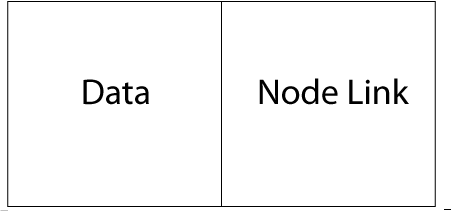
\includegraphics[height=1in]{node.png}
\end{center}
\end{column}
\begin{column}{2.75in}
\begin{lstlisting}[language=Java, frame=none]
private class Node {
  public Object data;
  public Node next;

  public Node(Object data, Node next) {
    this.data = data;
    this.next = next;
  }
}
\end{lstlisting}
\end{column}
\end{columns}


\end{frame}
%------------------------------------------------------------------------

%------------------------------------------------------------------------
\begin{frame}[fragile]{Singly Linked Lists}


A singly linked list
\begin{itemize}
\item Contains a pointer to a ``head'' node ({\tt null} if empty).
\item The head node's {\tt next} points to the second node, the second node's {\tt next} points to the third node, and so on.
\item The {\tt next} reference of the last node is {\tt null}
\end{itemize}

Here's a depiction of the nodes in a singly linked list with three elements:
\begin{center}
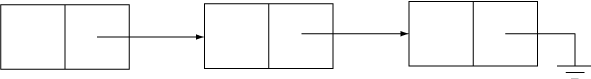
\includegraphics[width=4.75in]{singly-linked-list.png}
\end{center}


\end{frame}
%------------------------------------------------------------------------

%------------------------------------------------------------------------
\begin{frame}[fragile]{Adding Elements to a Singly Linked List}

\vspace{-.075in}
1. Create a new {\tt Node}.
\vspace{-.05in}
\begin{center}
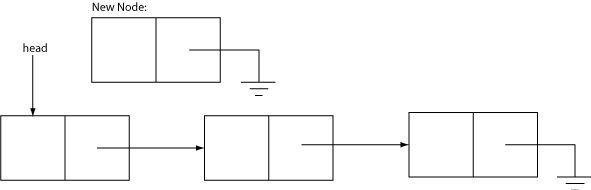
\includegraphics[height=.75in]{add-linked-list-1.png}
\end{center}

\vspace{-.05in}
2. Set the {\tt next} reference of the new {\tt Node} to the current {\tt head}.
\vspace{-.05in}
\begin{center}
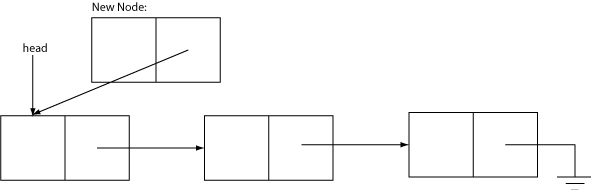
\includegraphics[height=.75in]{add-linked-list-2.png}
\end{center}
\vspace{-.05in}
3. Set the {\tt head} reference to the new {\tt Node}
\begin{center}
\vspace{-.05in}
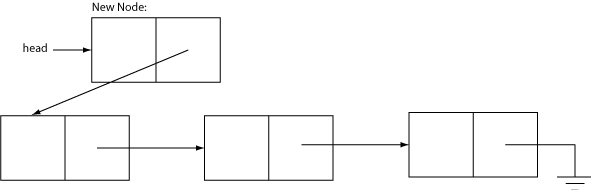
\includegraphics[height=.75in]{add-linked-list-3.png}
\end{center}

See \link{\code/data-structures/LinkedList.java}{LinkedList.java} for the code.

\end{frame}
%------------------------------------------------------------------------
%------------------------------------------------------------------------
\begin{frame}[fragile]{Finding an Item in a Linked List}


An algorithm for finding an item in a linked list:
\begin{lstlisting}[language=Java]
foundNode: Node := null
currentNode: Node := LinkedList.head
while currentNode != null && foundNode = null
    if currentNode.data = queryItem
        foundNode := currentNode
    currentNode := currentNode.next
\end{lstlisting}

The postcondition of this algorithm is that {\tt foundNode} will be:

\begin{itemize}
\item The node containing the query item, or
\item {\tt null} if the query item is not in the list.
\end{itemize}


\end{frame}
%------------------------------------------------------------------------

%------------------------------------------------------------------------
\begin{frame}[fragile]{Inserting Elements into a Linked List}
\vspace{-.1in}
1. Find the existing {\tt Node} to insert new element after.\\
2. Create a new {\tt Node}.
\vspace{-.2in}
\begin{center}
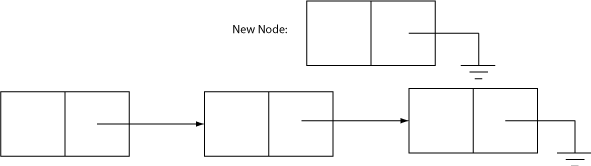
\includegraphics[height=.7in]{insert-linked-list-1.png}
\end{center}

\vspace{-.05in}
3. Set the {\tt next} reference of the new {\tt Node} to the {\tt next} reference of the existing node.
\vspace{-.2in}
\begin{center}
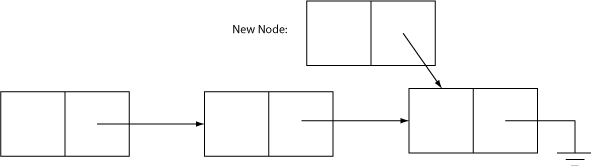
\includegraphics[height=.7in]{insert-linked-list-2.png}
\end{center}

\vspace{-.05in}
4. Set the {\tt next} reference of the existing node to the new {\tt Node}.
\begin{center}
\vspace{-.05in}
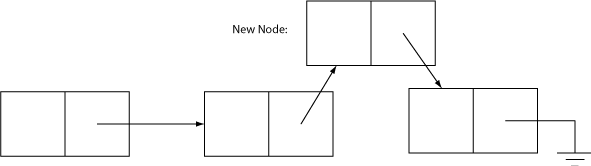
\includegraphics[height=.7in]{insert-linked-list-3.png}
\end{center}

See \link{\code/LinkedList.java}{LinkedList.java} for the code.

\end{frame}
%------------------------------------------------------------------------

%------------------------------------------------------------------------
\begin{frame}[fragile]{Computing the Length of a Linked List}


An algorithm for computing the length a linked list:
\begin{lstlisting}[language=Java]
length: int := 0
currentNode: Node := LinkedList.head
while currentNode != null
    length := length + 1
    currentNode := currentNode.next
\end{lstlisting}

The postcondition of this algorithm is that {\tt length} will be equal to the number of nodes in the list.


\end{frame}
%------------------------------------------------------------------------

%------------------------------------------------------------------------
\begin{frame}[fragile]{Generic Linked Lists}


To make our LinkedList generic we only need to add a type parameter to the declaration:
\begin{lstlisting}[language=Java]
public class GenericLinkedList<E> { ...
\end{lstlisting}

and replace {\tt Object} with {\tt E} in the body of the class.

See \link{\code/data-structures/GenericLinkedList.java}{GenericLinkedList.java}

\end{frame}
%------------------------------------------------------------------------

%------------------------------------------------------------------------
\begin{frame}[fragile]{Doubly Linked Lists}


A doubly linked list simply adds a {\tt previous} reference to the {\tt Node} class so that the list can be traversed forwards or backwards.
\begin{lstlisting}[language=Java]
    private class Node<E> {
        E data;
        Node<E> next;
        Node<E> previous;

        public Node(E data, Node<E> next, Node<E> previous) {
            this.data = data;
            this.next = next;
            this.previous = previous;
        }
    }
\end{lstlisting}

Doubly linked lists work the same, except that the algorithms for inserting and removing items requires a bit more link fiddling (have to set previous links as well).

See \link{\code/data-structures/DoublyLinkedList.java}{DoublyLinkedList.java}.

\end{frame}
%------------------------------------------------------------------------

%------------------------------------------------------------------------
\begin{frame}[fragile]{Programming Exercises}

Programming Exercise 1
\begin{itemize}
\item Add a {\tt get(int index)} method to {\tt GenericLinkedList}.
\item Add a {\tt remove(T item)} method to {\tt GenericLinkedList}.
\end{itemize}
Programming Exercise 2
\begin{itemize}
\item Implement {\tt public static int binarySearch(int[] a, int v)}.  Return -1 if {\tt v} is not in {\tt a}.
\item Bonus: implement {\tt public static <T> int binarySearch(T[] a, T v, Comparator<? super T> c)}. Return -1 if {\tt v} is not in {\tt a}.
\item Bonus: for either of the options above, implement your method using a recursive helper method.
\item Bonus question: if we wanted to implement a similar method for a {\tt Collection}, how would we do it?  Could we define such a binary search method for any {\tt Collection}?
\item Bonus question 2: what is the running time (Big-O) of binary search?
\end{itemize}


\end{frame}
%------------------------------------------------------------------------

% %------------------------------------------------------------------------
% \begin{frame}[fragile]{}


% \begin{lstlisting}[language=Java]

% \end{lstlisting}

% \begin{itemize}
% \item
% \end{itemize}


% \end{frame}
% %------------------------------------------------------------------------


\end{document}
